\chapter{統計學概論}
    在這個資料取得越來越容易的時代，各個領域都希望能夠分析手上的資料、獲得結論並進行決策。例如在醫療領域中，我們常想知道一個療法對於病患的預後是否有影響，以進行後續補助政策的制定或治療指引的撰寫；或是能不能夠利用病患的影像資料、抽血資料和病史預測疾病的發生率，以達到提前篩檢、早期診斷、早期治療的目的。因此，如何有效率地整理資料、去蕪存菁、並進行合乎科學原理的分析便成為一門顯學。統計便是一門利用科學方法來處理並分析資料的學科。當今因為資訊計算能力的超指數成長，分析整理資料的方法種類和複雜度也呈現爆炸性的增長，但這些方法的目的仍然是探尋資料內部隱含的資訊，因此背後仍然是以統計架構為基石。本課程前半段將著重統計觀念的建立，包含為什麼需要利用統計方法分析資料，以及推論統計的邏輯基礎。後半段則將介紹常用的統計檢定與回歸方法，並輔以因果推論的理論框架介紹，以期了解如何針對有興趣的研究議題，選擇適當的統計模型並解讀分析結果。在本章，我們會簡介統計學的發展歷史，並帶出統計學的兩大分支：敘述性和推論性統計。針對推論性統計，我們還會探討母體、抽樣和樣本的概念，以及這些概念如何融合到推論性統計的流程中。

\begin{introduction}[第 \thechapter 章學習目標]{1}
    \item 敘述性統計和推論性統計的目的
    \item 母體、樣本和抽樣的概念
    \item 推論性統計的流程與背後假設
    \item 統計推論的初步評讀
\end{introduction}

\section{統計的分支：敘述性統計}
    相較於其他領域，統計是一門十分近代才成型的學科，約十八世紀才開始發展。統計的英文是 \textit{statistics}，拉丁字源為 \textit{statisticum}，意謂「政府的」，因為統計最初是政府用來處理國家級資料（例如人口、經濟），以幫助管理國家的方法。首度將 \textit{statistics} 這個字引入英文的人據傳是蘇格蘭的 Sir John Sinclair (1754-1835)。他編纂了一本共有 22 集的 \textit{Statistical Account of Scotland}，記錄了當時蘇格蘭的各式資料，包括地理、人口、農工生產等等，且紀錄內容並不限於數字。例如圖\ref{fig:john_sinclair}所示，書中內容記錄了其中一個地區的人口職業分布，還提到當地的道路狀況。

\begin{figure}[htbp]
  \centering
  \includegraphics[width=0.9\textwidth]{figures/01-Overview/john_sinclair.png}
  \caption{Sir John Sinclair (1754-1835) 與 \textit{Statistical Account of Scotland} 的內頁}
  \label{fig:john_sinclair}
\end{figure}

    類似 \textit{Statistical Account of Scotland} 這類將資料整理後，以易懂的圖表呈現的方式一般被稱為\textit{敘述性統計} (descriptive statistics)。敘述統計學能將相對大量的資料精簡為具有代表性的統計數據（例如比例、平均值、中位數等敘述統計量）或是圖片，以幫助我們快速了解資料的特性與隱含的訊息。運用得當的敘述統計方法能夠讓決策者根據資料帶來的訊息即時地做出決策。例如，1854 年倫敦蘇活區 (Soho) 霍亂大爆發。該時代對於霍亂的病原為何仍然莫衷一是，但內科醫師 John Snow (1813-1858) 猜想霍亂的病原可能來自於水，因此根據蘇活區霍亂病例在家戶的分布做了圖 \ref{fig:john_snow}，其中同一家戶的病例數越多，長條圖就越長。John Snow 發現霍亂病例似乎有以圖中的紅點為中心群聚分布的趨勢，而該紅點標記的是蘇活區的一個公用抽水幫浦，和 John Snow 猜想的水媒傳染相符合。當地市政府而後也決定將抽水幫浦的手柄移除。John Snow 則因一系列霍亂相關的研究而被譽為「流行病學之父」。從這個圖片可以看出，John Snow將病例用散佈圖的方式標記是明智之舉。如果單純調查各分區的病例數而未作圖，則不見得能發現地理位置的群聚現象。更多內容，請詳見 \href{https://www.youtube.com/watch?v=VJ86D_DtyWg}{影片}。

    \begin{figure}[htbp]
      \centering
      \includegraphics[width=0.9\textwidth]{figures/01-Overview/john_snow.png}
      \caption{John Snow (1813-1858)、其繪製的霍亂地圖、及地圖中心的公用抽水幫浦}
      \label{fig:john_snow}
    \end{figure}

    \begin{figure}[htbp]
      \centering
      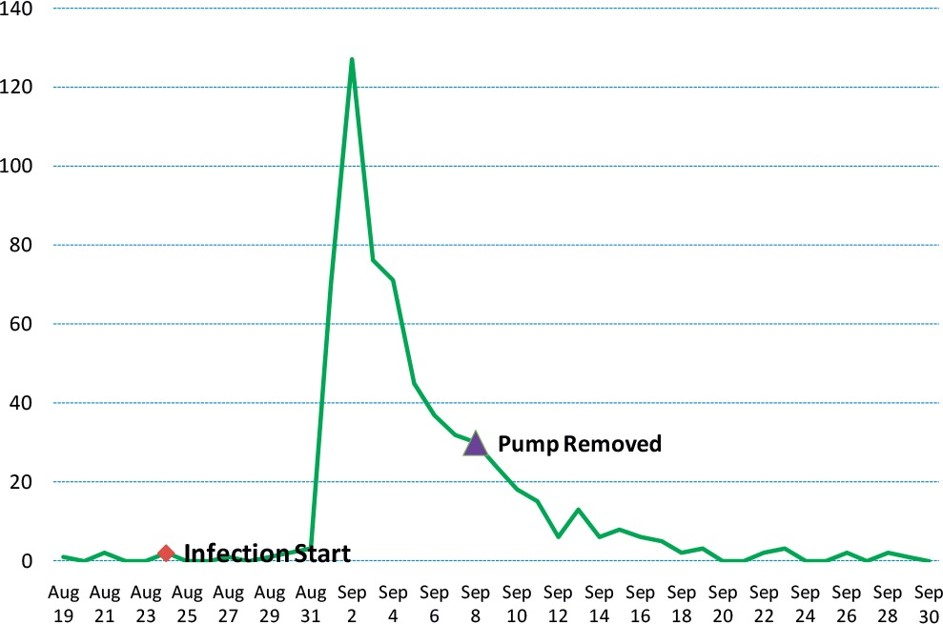
\includegraphics[width=0.725\textwidth]{figures/01-Overview/cholera_death.jpg}
      \caption{1854 年倫敦霍亂流行期間 Broad Street 附近的死亡數統計}
      \label{fig:cholera_death}
    \end{figure}
    
    \bigskip
    
    \begin{custom}{動動腦}
        從 John Snow 繪製的圖片，是否已經足夠證明水就是霍亂的傳播根源？後來市政府將抽水幫浦的手柄移除，同時間霍亂疫情也逐漸緩和，如圖 \ref{fig:cholera_death} 所示。如此是否已經足夠證明水就是霍亂的傳播根源？
    \end{custom}

    \answerbox{150pt}
    
    
\section{統計的分支：推論性統計}

    有了敘述統計學後，決策者理論上即可根據圖像或敘述統計量來做決策。例如，利用健保資料庫了解國人糖尿病的患病率後，即可用「患病率」這個敘述統計量估算糖尿病相關照護計畫的預算。然而，很多時候因為資源的限制，我們沒有辦法針對有興趣的目標量取得所有的資料。舉例而言，假設我們有一個針對肺腺癌的新藥，並想要了解當前台灣第三期肺腺癌的病人服用該藥的副作用發生率（我們簡寫為 $p$）。理想上，我們想要搜集所有第三期肺腺癌的病人，都給予新藥後，評估出現副作用的比例。然而，這樣的作法在金錢資源上和倫理上都行不通。

    \smallskip
    
    針對這個問題，一個可行的替代方法是，我們可以募集 $50$ 位第三期肺腺癌的病人，並給予新藥後，評估這 $50$ 位病人出現副作用發生率。比方說有 $2$ 位出現副作用，此時這 $50$ 位肺腺癌病人的副作用發生率為 $4\%$。只要我們募集的病人具有代表性，那麼「當前台灣第三期肺腺癌病人」的副作用發生率 $p$ 應該會和這 $50$ 位肺腺癌病人類似，也就是大約 $4\%$。然而，$p$ 顯然不太可能剛剛好是 $4\%$，因為這個算出來的 $4\%$ 會隨著募集到的病患不同而變動：如果重新募集另外兩組 $50$ 位病人，發生副作用的人數可能因為隨機性而變成 $1$ 人或 $3$ 人，進而算得 $2\%$ 或 $6\%$ 的發生率。因此，我們只知道 $p$ 應該在 $4\%$ 左右，但是它的實際數值則因為隨機的變動而有\textit{不確定性}。因此，統計學家引進了機率論來描述並處理不確定性，因而衍生出\textit{推論性統計}（Inferential statistics）。
    
    在推論性統計中，有幾個名詞是我們必須需要熟悉的。我們條列如下，並以上述例子作為對照：

    \begin{itemize}
        \item \textit{母體} (Population)：我們實際上有興趣的總群體，「當前台灣第三期肺腺癌的病人」。
        \item \textit{參數} (Parameter)：我們有興趣的目標量，「肺腺癌病人接受新藥的副作用發生率 $p$」。
        \item \textit{抽樣} (Sampling)：從母體抽取一部份個體的過程。
        \item \textit{樣本} (Sample)：從母體抽出的一組個體，「$50$ 位第三期肺腺癌病人」。
        \item \textit{樣本數} (Sample size)：樣本的個體數，「$50$」。
        \item \textit{參數估計式} (Parameter estimator)：根據我們對母體的假設及抽樣方法，建構出一個估計參數的方法，「樣本中發生副作用的人數除以樣本數」。
        \item \textit{參數估計量} (Parameter estimate)：把樣本帶入參數估計式得到的數值，「$4\%$」。
    \end{itemize}

    隨後，根據圖\ref{fig:flowchart}的流程，我們可以利用推論性統計的技巧，根據抽樣方法和母體假設對參數做推論，並且以量化的語言說明結果。例如：「當前台灣第三期肺腺癌病人服用新藥之副作用發生率的 $95\%$ 信賴區間為 $(0.49\%, 13.71\%)$」、「在 $5\%$ 的顯著水準下，沒有足夠證據顯示當前台灣第三期肺腺癌病人服用新藥的副作用發生率大於 $1\%$」等等。以上的敘述現在看起來可能不知所云，但後續課程將詳細介紹推論性統計的解讀方法，而後我們就會知道這些推論背後的意義，以及為什麼要弄得那麼複雜。

    \smallskip
    
    圖\ref{fig:flowchart}的流程也給我們一個檢視統計推論中每個環節是否正確的藍圖。例如，針對公共議題的民意調查，如果只在火車站附近作隨機街訪，則樣本來源都只來自活動於火車站附近的國民，而可能無法代表我們預想的「全民」母體。針對心血管疾病發病率的預測模型，如果建模資料來自於高階健檢的檢查資料，則該預測模型可能無法外推到一般民眾使用。進行氣喘急性發作危險因子的分析時，如果單一病患因多次發作而提供多筆資料，但是使用的分析方法卻假設抽樣得到的樣本是互不相關，那麼得到的推論結果就會有訛誤。而且我們可以看到，推論統計能夠做的只是根據母體假設以及抽樣方法儘量建構好的參數估計方法、並針對這些估計提供不確定性的度量。但如果母體假設有誤、抽樣流程不正確、或欲推論的目標群體和母體不一致，那麼統計能夠幫忙的程度就非常有限。更有甚者，如果隨意使用統計方法並報告結果，可能會導致推論謬誤，不可不慎。

    \bigskip
    
    \begin{figure}[htbp]
      \centering
      \includegraphics[width=0.9\textwidth]{figures/01-Overview/flowchart.png}
      \caption{推論統計的流程架構}
      \label{fig:flowchart}
    \end{figure}
    
    \bigskip
    
    \begin{custom}{動動腦}
        現今健保資料庫的覆蓋率已經超過 99.7\%。如果以台灣民眾為母體，那麼健保資料庫等同幾乎收集了母體的所有資料。在這個情況下，還有推論統計的必要嗎？
    \end{custom}
        
    \answerbox{200pt}

    \pagebreak
    
    \begin{custom}{動動腦}
        在問卷調查中（例如：調查對某政策的支持與否），經常會出現某些題目漏答或拒答的現象。在以下的假設情境下，是否能用有回答的問卷估計出正確的政策支持率？(1) 漏(拒)答是完全隨機的，和受訪者的任何特性均無關；(2) 漏(拒)答不是完全隨機的，且和受訪者支不支持政策有關；(3) 漏(拒)答並非完全隨機，但僅和受訪者的性別、年齡有關，且問卷中有詢問性別及年齡；(4) 漏(拒)答並非完全隨機，但僅和受訪者的教育程度有關，但問卷未詢問教育程度。
    \end{custom}

    \answerbox{200pt}
    
\section{統計學的獨立發展}

統計學的雛型雖然從十八世紀萌芽，並接受數學機率論的薰陶而逐漸茁壯，但直到十九世紀末，統計學才作為一門獨立的學門進行系統性的發展。其中最重要的推手是遺傳學家 Francis Galton (1822-1911)。Galton 是位極具傳奇色彩的學者，兼具遺傳學家、地理學家、氣象學家、發明家種種角色。Galton 發明的指紋分類系統至今仍在犯罪學中使用。Galton 受到同為遺傳學家的遠房表兄 Charles Darwin 以及其 1859 年發表的開創性著作《\textit{物種起源}》(On the Origin of Species) 的影響，對於連續性狀如身高、智力的遺傳十分感興趣。Galton 試圖用數學模型來分析並描述這些性狀的遺傳特性，因而發展出了回歸、相關性等等統計學最基本的概念。其中「回歸」的發現來自一個有趣的觀察：Galton 取得了數百個家庭中父母與成年子女的身高數據，發現高個子父母的子女雖然也傾向較高，但就百分位而言會不如父母來得極端，也就是會「回歸」到人群的平均身高；矮個子父母的子女也有類似現象。Galton 稱此現象為「向平庸回歸」(regression toward mediocrity)，也造就了「回歸」一詞的由來。雖然這個由來現在聽起來有些負面，但它描述的統計現象卻極為深刻。這促成了標準差、回歸和相關等基本統計概念的發展。有關向平均回歸的議題，請參見\href{https://www.youtube.com/watch?v=lOWjRaCKbQg}{連結}。

\medskip

Karl Pearson (1857-1936) 作為高爾頓的學生（及被贊助者），將高爾頓的直覺性想法轉化為嚴謹的數學架構，並完善了回歸和相關的數學框架，提出了卡方檢定和主成分分析等統計方法。而後，Ronald Fisher (1890-1962) 大力推進了遺傳以及推論統計的數學理論，並基於農業研究提出實驗設計法以及其統計分析，如變異數分析 (analysis of variance)。有趣的是，Fisher 還重新分析了 Mendel 的豌豆實驗數據，並發現數據「太完美」，懷疑可能經過潤飾，成為科學史上的一樁懸案。費雪也是位性格鮮明的人物。他堅持吸菸，甚至在晚年還公開抨擊吸菸與肺癌有因果關係的流行病學證據不夠嚴謹，成為他學術生涯的一大爭議。

\medskip

Galton、Pearson 和 Fisher 三人為當代推論性統計打下了重要基礎。但這些統計學巨人大多與優生學 (eugenics) 有複雜的關聯。Galton 創立了優生學，Pearson 和 Fisher 也都曾支持這個當時被視為「科學」的運動，因此當今在倫理層面上也引發許多討論。例如 University College London 在 2020 年就因 Galton 與優生學的關聯而將 Galton Lecture Theatre 改名為 Lecture Theatre 115。

    \begin{figure}[htbp]
      \centering
      \includegraphics[width=0.9\textwidth]{figures/01-Overview/statisticians.png}
      \caption{奠基統計學的統計學家：（左至右）Francis Galton, Karl Pearson, William Gosset, Ronald Fisher}
      \label{fig:statisticians}
    \end{figure}

\begin{takehome}
    \item 敘述統計旨在以數字或圖形彙整資料，以便於資料的檢視與理解。
    \item 推論統計旨在從樣本中估計並推論未知的母體參數，並將抽樣所帶來的隨機性納入考量。
    \item 統計推論需綜合母體假設、抽樣方法、估計式、以及估計值之資訊。
    \item 當樣本不具母體之代表性時，使用統計方法進行統計推論可能會得到錯誤的結論。
\end{takehome}